\documentclass[a4paper,11pt]{article}
\usepackage[utf8]{inputenc}
\usepackage[french]{babel}
\usepackage{amsmath}
\usepackage[osf,sups]{Baskervaldx} % lining figures
\usepackage[bigdelims,cmintegrals,vvarbb,baskervaldx,frenchmath]{newtxmath} % math font
%\usepackage[cal=boondoxo]{mathalfa} % mathcal from STIX, unslanted a bit
%\usepackage{float}
\usepackage{graphicx}
\usepackage{url,hyperref}
%\usepackage{color}

\setlength{\parindent}{0em}
\setlength{\parskip}{1em}
%\addtolength{\hoffset}{-3.5em}
%\addtolength{\textwidth}{7em}
%\addtolength{\voffset}{-5em}
%\addtolength{\textheight}{10em}

%\addtolength{\voffset}{-6em}
%\addtolength{\textheight}{12em}

\begin{document}

{\Large how to compute the sound of a xylophone}

%The goal of this work is to write the simplest possible code that predicts the
%timbre of percussion and wind instruments.
%
%\bigskip

We model three-dimensional objects as subgraphs of a 3D grid graph.
For simplicity of the visualization we start with the 2D case, where we can
model subsets as binary images.

%RUN_VERBATIMS octavescript

First we build the basic ``bar'' shape, which is a rectangle minus a disk.

\begin{verbatim}
# characteristic function of a bar centered at the origin
function m = bar(
                     a, b,  # width, height of the rectangle
                     d,     # vertical offset of the disk center
                     r,     # radius of the disk
                     x, y   # point where the function is evaluated
                   )
        m = (abs(x)<a) & (abs(y)<b) & (hypot(x,y-d)>r);
end
\end{verbatim}

\begin{verbatim}
# characteristic function of a tilted and rotated bar
function m = rbar(
                       a, b, d, r, x, y,  # same parameters as above
                       alpha,             # tilt coefficient
                       theta              # rotation angle
                     )
        X = cos(theta) * x - sin(theta) * y;
        Y = sin(theta) * x + cos(theta) * y;
        m = bar(a, b, d, r, X, alpha * Y);
end
\end{verbatim}

\begin{verbatim}
# characteristic function of a tilted and rotated bar (discrete image)
function m = rbar_image(
                            a, b, d, r, alpha, theta,  # as above
                            n                          # number of samples
                          )
        [x,y] = meshgrid(linspace(-1,1,n), linspace(-1,1,n));
        m = rbar(a, b, d, r, x, y, alpha, theta);
end
\end{verbatim}

\begin{verbatim}
# try the code above
w = 128;
M = rbar_image(.9, .4,  .5, .4,  1, pi/3,   w);
imwrite(M, "f/bar.png")
\end{verbatim}


\includegraphics{f/bar.png}\verb+bar.png+

\begin{verbatim}
# build the incidence matrix of a grid graph
function B = grid_incidence(w, h)                          # grid graph WxH
        x = sparse(1:w-1, 2:w, 1, w-1, w) - speye(w-1,w);  # path of length W
        y = sparse(1:h-1, 2:h, 1, h-1, h) - speye(h-1,h);  # path of length H
        B = [ kron(speye(h),x) ; kron(y,speye(w)) ];       # kronecker union
end
\end{verbatim}

\begin{verbatim}
# build a grid graph (whole space) and the laplacian of shape M
B = grid_incidence(w, w);
P = speye(w*w, w*w)(find(M(:)),:); # binary weights
PB = B*P';                         # weighted first derivative
L = -PB' * PB;                     # laplacian matrix (second derivative)
\end{verbatim}

\begin{verbatim}
# study the vibration modes of this shape
[V,D,flag] = eigs(-L, 40, "be");   # compute both ends of the eigensystem
v1 = P'*V(:,1);
v2 = P'*V(:,2);
v3 = P'*V(:,3);
v4 = P'*V(:,4);
v5 = P'*V(:,5);
v6 = P'*V(:,6);
v7 = P'*V(:,7);
v8 = P'*V(:,8);
v9 = P'*V(:,9);
v10 = P'*V(:,10);
v11 = P'*V(:,11);
v12 = P'*V(:,12);
v13 = P'*V(:,13);
v14 = P'*V(:,14);
v15 = P'*V(:,15);
v16 = P'*V(:,16);
v17 = P'*V(:,17);
v18 = P'*V(:,18);
v19 = P'*V(:,19);
v20 = P'*V(:,20);
vm1 = P'*V(:,20);
vm2 = P'*V(:,19);
vm3 = P'*V(:,18);
vm4 = P'*V(:,17);
vm5 = P'*V(:,16);
vm6 = P'*V(:,15);
imwrite(reshape(255*(v1-min(v1))/(max(v1)-min(v1)),w,w), "f/marimba_v1.png")
imwrite(reshape(255*(v2-min(v2))/(max(v2)-min(v2)),w,w), "f/marimba_v2.png")
imwrite(reshape(255*(v3-min(v3))/(max(v3)-min(v3)),w,w), "f/marimba_v3.png")
imwrite(reshape(255*(v4-min(v4))/(max(v4)-min(v4)),w,w), "f/marimba_v4.png")
imwrite(reshape(255*(v5-min(v5))/(max(v5)-min(v5)),w,w), "f/marimba_v5.png")
imwrite(reshape(255*(v6-min(v6))/(max(v6)-min(v6)),w,w), "f/marimba_v6.png")
imwrite(reshape(255*(vm1-min(vm1))/(max(vm1)-min(vm1)),w,w), "f/marimba_vm1.png")
imwrite(reshape(255*(vm2-min(vm2))/(max(vm2)-min(vm2)),w,w), "f/marimba_vm2.png")
imwrite(reshape(255*(vm3-min(vm3))/(max(vm3)-min(vm3)),w,w), "f/marimba_vm3.png")
iio_write("f/marimba_v01.tiff", reshape(v1,w,w));
iio_write("f/marimba_v02.tiff", reshape(v2,w,w));
iio_write("f/marimba_v03.tiff", reshape(v3,w,w));
iio_write("f/marimba_v04.tiff", reshape(v4,w,w));
iio_write("f/marimba_v05.tiff", reshape(v5,w,w));
iio_write("f/marimba_v06.tiff", reshape(v6,w,w));
iio_write("f/marimba_v07.tiff", reshape(v7,w,w));
iio_write("f/marimba_v08.tiff", reshape(v8,w,w));
iio_write("f/marimba_v09.tiff", reshape(v9,w,w));
iio_write("f/marimba_v10.tiff", reshape(v10,w,w));
iio_write("f/marimba_v11.tiff", reshape(v11,w,w));
iio_write("f/marimba_v12.tiff", reshape(v12,w,w));
iio_write("f/marimba_v13.tiff", reshape(v13,w,w));
iio_write("f/marimba_v14.tiff", reshape(v14,w,w));
iio_write("f/marimba_v15.tiff", reshape(v15,w,w));
iio_write("f/marimba_v16.tiff", reshape(v16,w,w));
iio_write("f/marimba_v17.tiff", reshape(v17,w,w));
iio_write("f/marimba_v18.tiff", reshape(v18,w,w));
iio_write("f/marimba_v19.tiff", reshape(v19,w,w));
iio_write("f/marimba_v20.tiff", reshape(v20,w,w));
iio_write("f/marimba_V1.tiff", reshape(vm1,w,w));
iio_write("f/marimba_V2.tiff", reshape(vm2,w,w));
iio_write("f/marimba_V3.tiff", reshape(vm3,w,w));
iio_write("f/marimba_V4.tiff", reshape(vm4,w,w));
iio_write("f/marimba_V5.tiff", reshape(vm5,w,w));
iio_write("f/marimba_V6.tiff", reshape(vm6,w,w));
\end{verbatim}


\includegraphics[width=0.15\linewidth]{f/marimba_v01.png}\verb+v01+\\

\includegraphics[width=0.15\linewidth]{f/marimba_v02.png}\verb+v02+\\
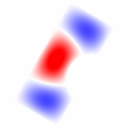
\includegraphics[width=0.15\linewidth]{f/marimba_v03.png}\verb+v03+\\

\includegraphics[width=0.15\linewidth]{f/marimba_v04.png}\verb+v04+\\

\includegraphics[width=0.15\linewidth]{f/marimba_v05.png}\verb+v05+\\

\includegraphics[width=0.15\linewidth]{f/marimba_v06.png}\verb+v06+\\
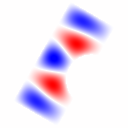
\includegraphics[width=0.15\linewidth]{f/marimba_v07.png}\verb+v07+\\
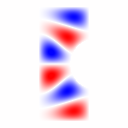
\includegraphics[width=0.15\linewidth]{f/marimba_v08.png}\verb+v08+\\
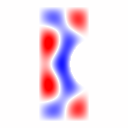
\includegraphics[width=0.15\linewidth]{f/marimba_v09.png}\verb+v09+\\
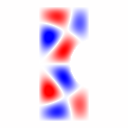
\includegraphics[width=0.15\linewidth]{f/marimba_v10.png}\verb+v10+\\
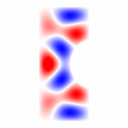
\includegraphics[width=0.15\linewidth]{f/marimba_v11.png}\verb+v11+\\
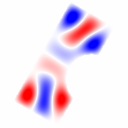
\includegraphics[width=0.15\linewidth]{f/marimba_v12.png}\verb+v12+\\
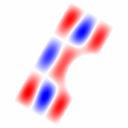
\includegraphics[width=0.15\linewidth]{f/marimba_v13.png}\verb+v13+\\
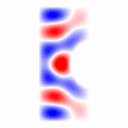
\includegraphics[width=0.15\linewidth]{f/marimba_v14.png}\verb+v14+\\
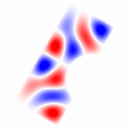
\includegraphics[width=0.15\linewidth]{f/marimba_v15.png}\verb+v15+\\
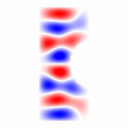
\includegraphics[width=0.15\linewidth]{f/marimba_v16.png}\verb+v16+\\
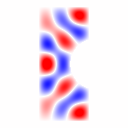
\includegraphics[width=0.15\linewidth]{f/marimba_v17.png}\verb+v17+\\
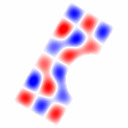
\includegraphics[width=0.15\linewidth]{f/marimba_v18.png}\verb+v18+\\
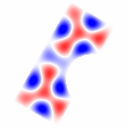
\includegraphics[width=0.15\linewidth]{f/marimba_v19.png}\verb+v19+\\
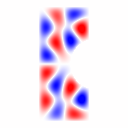
\includegraphics[width=0.15\linewidth]{f/marimba_v20.png}\verb+v20+\\

\end{document}


% vim:set tw=79 spell spelllang=fr:
